\chapter{Das Referenzmodell: Einzelne Kugel auf festem Grund}



\section{Erstellung und Equilibrierung der Probe}
	Eine Probe im Sinne der MD ist eine Datei, welche mindestens alle notwendigen Eigenschaften
	aller Teilchen im System speichert. Dazu gehören natürlich der Ort und die Geschwindigkeit
	jedes Teilchens, aber auch der Teilchentyp und die Teilchenmasse. Der Mulde im LJ-Potential
	\eqref{eq:potential_lj} nach gibt es für alle Teilchen einen Zustand minimaler Energie.
	Aus diesem Grund existiert ein stationärer Gleichgewichtszustand (\emph{Equilibrium}). Den
	Gesetzen der Thermodynamik folgend geht jedes ungestörte Nichtgleichgewichtssystem in sein
	Equilibrium über. Dieser Vorgang heißt \emph{Equilibrierung}. Da eine Probe prinzipiell einen
	beliebigen Zustand haben kann, ist eine \emph{vorherige} Equilibrierung besonders wichtig.
	Andernfalls findet der Equilibrierungsprozess gestört während der eigentlichen Simulation
	statt, was zu verfälschten Ergebnissen führen kann.

	Für das Modell dieser Arbeit bietet es sich an, eine auf \SI{300}{\kelvin} aufgeheizte Probe
	zu betrachten. Viele der in der Literatur auffindbaren Vergleichswerte zu Materialkonstanten
	werden bei diesem der Raumtemperatur nahe gelegenen Wert angegeben. Zudem bildet diese
	Temperatur das Problem gut ab.

	\subsection{Homogene Deformation}
		Um eine Probe nun in ihren Gleichgewichtszustand mit dieser Temperatur zu versetzen bietet
		es sich an, zuerst eine Probe der Temperatur \SI{0}{\kelvin} zu erstellen und diese dann
		aufzuheizen. Der rechnerische Nullpunkt lässt sich einfach dadurch erreichen, dass die
		Teilchengeschwindigkeiten auf 0 gesetzt werden. Mithilfe einer homogenen Deformation wird
		eine Simulation ohne Berücksichtigung der durch die Kraft verursachten Teilchenbewegungen
		durchgeführt. In jedem Simulationsschritt wird die Probe mithilfe einer zum Gitter
		achsenparallel wirkenden Deformationsmatrix inkrementell skaliert. Der sich dadurch
		ergebende Verlauf der mittleren potentiellen Energie kann nun minimiert werden. Aufgrund
		der Proportionalität zwischen dem Druck und den gemittelten Kräften äußert sich diese
		Stelle in Abbildung \ref{fig:homdef} in Form einer Nullstelle genau dort, wo die
		potentielle Energie minimal ist. Dies ist auch in sofern einleuchtend, da der Druck
		angibt, inwiefern sich einen Probe beim loslassen zusammenziehen oder ausdehnen würde
		\cite{rapp2014laserablation}.

		\begin{figure}[!ht]
			\centering
			\includegraphics[width=0.9\textwidth]{chapter/main/single/plt/equilibration/homdef.eps}
			\caption{Die mittlere potentielle Energie und der Probendruck aufgetragen gegen das
			Volumen pro Teilchen. Das Energieminimum kann durch einen näherungsweise quadratischen
			Fit um das Minimum der potentiellen Energie oder über eine Nullstellensuche des Druck
			bestimmt werden. In diesem Fall liegt das Energieminimum bei einem Teilchenvolumen von
			\SI{16.38}{\angstrom\cubed}.}
			\label{fig:homdef}
		\end{figure}

	\subsection{Aufheizen der Probe}
		Die bisherige Simulation fand unter Beachtung der Regeln eines mikrokanonischen Ensembles
		(\emph{NVE}) statt. Das bedeutet, dass neben der Teilchenzahl $N$ und dem Volumen $V$ die
		Gesamtenergie $E$ festgehalten wurde. Da im nächsten Schritt eine Temperaturerhöhung zum
		Aufheizen der Probe notwendig ist, ist ein NVE-Ensemble System so zwangsläufig ungeeignet.
		Stattdessen bietet sich das kanonische Ensemble (\emph{NVT}) an. Hier werden auch die
		Teilchenzahl und das Volumen fest gesetzt, allerdings wird hier statt der Energie die
		Temperatur $T$ durch Kopplung an ein Wärmebad vorgegeben. In der Simulation wird dies
		mithilfe eines Thermostats realisiert. Ein Thermostat manipuliert dabei die Simulation in
		der Hinsicht, dass die Temperatur der Vorgabe entspricht. Ein einfacher Thermostat wäre
		das Berendsen-Thermostat, bei dem der durch das Äquipartitionstheorem
		\eqref{eq:equipartition} gegebene Zusammenhang zwischen Temperatur und
		Teilchengeschwindigkeit genutzt wird, um alle Teilchengeschwindigkeiten global zu
		reskalieren. Dies hat allerdings einen Verlust der Maxwell-Boltzmann-Verteilung der
		Geschwindigkeitsbeträge zur Folge. Das in IMD verwendete Thermostat ist deshalb das
		\emph{Nosé-Hoover-Thermostat} \cite{rapp2014laserablation}.

		\begin{figure}[!ht]
			\centering
			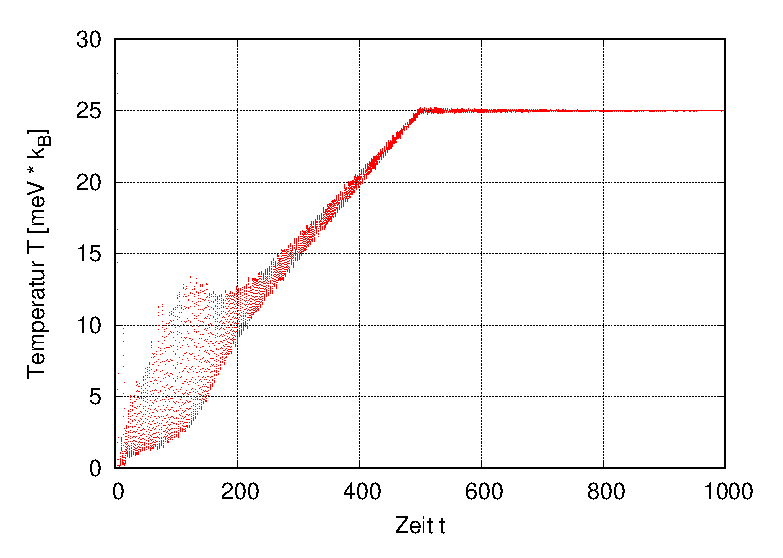
\includegraphics[width=0.9\textwidth]{chapter/main/single/plt/equilibration/thermostat.eps}
			\caption{Der Aufheizprozess mit vorgegebener Temperatur. Die Fluktuationen werden
			mit fortschreitender Zeit geringer.}
			\label{fig:thermostat}
		\end{figure}

		Abbildung \ref{fig:thermostat} zeigt das Aufheizen einer würfelförmigen Probe mithilfe des
		in IMD implementierten Nosé-Hoover-Thermostats. Während die Temperatur am Anfang trotz
		Vorgabe noch schwankt, vermindert sich dieser Effekt mit der Zeit. Ab ungefähr 800
		IMD-Zeiteinheiten sind die Fluktuationen in etwa konstant.

		\begin{figure}[!ht]
			\centering
			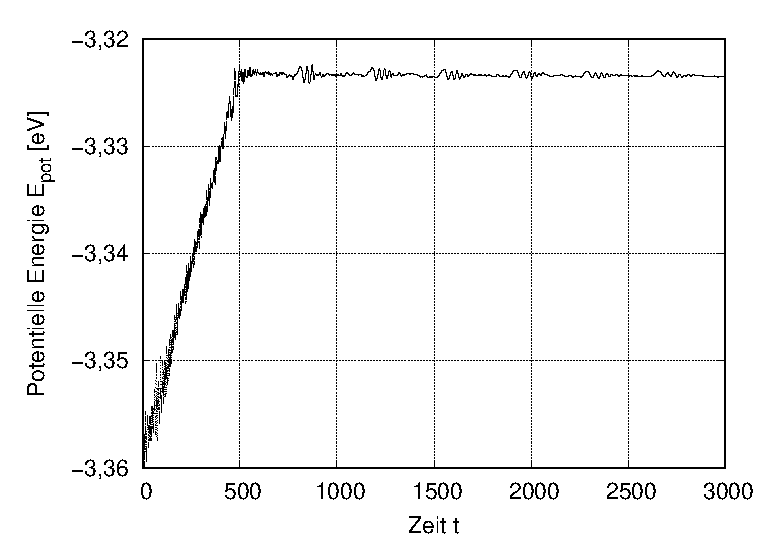
\includegraphics[width=0.9\textwidth]{chapter/main/single/plt/equilibration/thermostat_pot.eps}
			\caption{Die potentielle Energie zeigt einen zur Temperatur proportionalen Verlauf}
			\label{fig:thermostat_pot}
		\end{figure}

		Wie allerdings in Abbildung \ref{fig:thermostat_pot} zu sehen ist, verhält sich die
		potentielle Energie proportional zum Temperaturverlauf. Von daher ist es ratsam nach dem
		Aufheizen eine NVE-Simulation bis zum Equilibrium durchzuführen.

	\subsection{Erzeugen einer Kugelprobe}
		Üblicherweise sind Proben quaderförmig und bilden durch \emph{periodischen Randbedingungen}
		(\emph{PBC}) ein Gitter, welches teilweise Eigenschaften eines unendlich ausgedehnten
		Gitters imitiert. Im Rahmen dieser Arbeit sind jedoch Kugelformen unter der Einwirkung von
		Gravitation interessant, da sie so den Pulverpartikeln beim SLM-Verfahren sehr ähnlich
		sind. Die einfachste Methode zum Erzeugen einer solchen Probe ist die Wahl eines
		entsprechenden Gitterausschnitts, wobei die umliegenden Teilchen entfernt werden.
		Hierbei gilt zu beachten, dass die Kugel erst nach der homogenen Deformation freigestellt
		wird. Das hat den Grund, dass eine homogene Deformation das gesamte Teilchensystem
		skaliert. Ist der Radius der Kugel sehr genau bemaßt, ändert er sich signifikant während
		dieses Prozesses. Wichtig ist für die nachfolgenden Equilibrierungsschritte auf jeden
		Fall, dass diese nun unter Einfluss der Gravitation mit ausreichend Equilibrierungszeit
		erfolgen. So wird gewährleistet, dass die Kugel etwas absackt und sich somit in ihre der
		Form entsprechenden Ruhelage begibt. Abbildung \ref{fig:equilibrated_sample} zeigt dabei
		die Ruhelage eines kugelförmigen Gitterausschnitts mit einem Durchmesser von
		\SI{400}{\angstrom}. Zwischen fixiertem Boden und beweglicher Kugel vergrößert sich die
		Kontaktfläche durch die Wirkung der Gravitation.

		Es ist allgemein empfehlenswert, wenn die Kugel nicht direkt in den Einflussbereich der
		PBC positioniert wird. Um eine derartige Selbstbeeinflussung zu verhindern könnten die PBC
		deaktiviert werden, jedoch stellten sich diese für die Erstellung problemverwandter Proben
		als nützlich heraus. So kann beispielsweise eine bereits equilibrierte Simulationsbox
		mehrfach hintereinanderkopiert werden, um eine Reihe an Kugeln zu erhalten. Sofern diese
		ursprüngliche Probe mit PBC equilibriert wurde ist der Boden nahtlos wiederholbar.
		Dass das Resultat dann nicht equilibriert werden muss, spart vor allem bei größeren Proben
		Zeit.

		\begin{figure}[!ht]
			\centering
			\includegraphics[width=\textwidth]{chapter/main/single/img/equilibration/sphere.zoom.png}
			\caption{Eine vollständig equilibrierte Kugel aus Aluminiumatomen (grün) auf einem
			festen, unbeweglichen Untergrund (rot) vergrößert die Kontaktfläche unter dem eigenen
			Gewicht}
			\label{fig:equilibrated_sample}
		\end{figure}


\section{Variation der Laserleistung bei fester Lasergeschwindigkeit}
		Wie in Abschnitt \ref{subsec:approximation} bereits erläutert werden für dieses Modell
		teils Näherungen verwendet, die ein direktes Übertragen der Simulationsdaten auf
		experimentelle Messdaten anhand einer reinen Messgrößenumrechnung nahezu unmöglich machen.
		Zur Verifizierung des Modells bietet sich also ein überwiegend qualitativer Abgleich der
		Beobachtungen mit Ergebnissen von Experimenten an.

		%\begin{figure}[!ht]
		%	\centering
		%	\includegraphics[width=0.6\textwidth]{chapter/main/single/img/scheme_graph.png}
		%	\caption{Schematische Darstelllung der durch Laserleistung und Lasergeschwindigkeit
		%	gemeinsamen Wirkung \cite{metalam2018how}}
		%	\label{fig:sceme_graph}
		%\end{figure}
		%
		%Abbildung \ref{fig:sceme_graph} zeigt schematisch, wie die Lasergeschwindigkeit und
		%die Laserleistung zusammen wirken. Eine schlechte Abstimmung aufeinander begünstigt
		%Defekte, während es einen optimalen Bereich gibt, innerhalb dessen Defekte .
		%Bei guter Abstimmng der Parameter
		%untereinander ergibt sich ein Fenster, für das das Ergebnis als gut gilt. Anhand der Variation in der Simulation
		%können solche Zusammenhänge auf Teilchenebene betrachtet und deshalb besser verstanden
		%werden.

		Zuerst soll der Einfluss der Laserleistung untersucht werden. Dabei wird die
		Lasergeschwindigkeit auf einen festen Wert von \SI{10}{\angstrom} pro IMD-Zeiteinheit
		gesetzt. Für die Wahl dieser Geschwindigkeit war wichtig, dass mit dem gegebene Setup eine
		komplette SImulation innerhalb einer Walltime ausgeführt worden konnte. Nun werden
		verschiedene Leistungen durchsimuliert, um Referenzsimulationen zu erhalten, an denen sich
		weitere Untersuchungen orientieren können. Vorläufiges Ziel ist es, jeder Leistung bei
		dieser Geschwindigkeit ein Schmelzvermögen zuzuordnen.

		Dieses wird durch den Materialanteil der Probe, der nach der Simulation geschmolzen ist,
		charakterisiert. Als Entscheidungskriterium hierfür wird eine
		\emph{Common Neighbor Analysis} (\emph{CNA}) verwendet. Eine CNA ist dabei ein Hilfsmittel
		zur Erkennung und Benennung von Gitterstrukturen. Wenn also ein Atom im Aluminium, das
		bekanntermaßen eine fcc-Gitterstruktur hat, als Teil einer anderen Struktur erkannt wird,
		muss es sich in diesem Kontext zwangsläufig um geschmolzenes Aluminium handeln. Dies
		funktioniert im Großen und Ganzen erfahrungsgemäß sehr zuverlässig, jedoch darf nicht
		vergessen werden, dass Randatome (beispielsweise auf Oberflächen) aus geometrischen
		Gründen falsch erkannt werden können.

		\begin{figure}[!ht]
			\centering
			\begin{subfigure}{0.49\textwidth}
				\centering
				\includegraphics[width=\textwidth]{chapter/main/single/plt/power_calibration/cna_vel10_start.eps}
				\subcaption{Anfangsbereich}
				\label{fig:cna_vel10_start}
			\end{subfigure}
			\begin{subfigure}{0.49\textwidth}
				\centering
				\includegraphics[width=\textwidth]{chapter/main/single/plt/power_calibration/cna_vel10_rate.eps}
				\subcaption{Langzeitentwicklung}
				\label{fig:cna_vel10_rate}
			\end{subfigure}
			\caption{Anteil der Teilchen, die zum geschmolzenen Material zählen über die
			Simulationszeit. Der senkrechte graue Balken markiert den Zeitpunkt zu dem der Laser
			bereits mit Geschwindigkeit $v_\text{Laser} = \SI{10}{\angstrom}$ pro IMD-Zeiteinheit
			vollständig über die Probe gefahren ist.}
			\label{fig:cna_vel10}
		\end{figure}

		In Abbildung \ref{fig:cna_vel10} ist der Anteil des geschmolzenen Materials für
		verschiedene Laserleistungen $P$ über die Zeit aufgetragen. In Abbildung
		\ref{fig:cna_vel10_start} ist der Zeitbereich, direkt nachdem der Laser darübergefahren
		ist, vergrößert.
		Hier ist zu sehen, dass der Laser die Probe schlagartig aufschmilzt und der Anteil an
		geschmolzenem Material kurzzeitig konstant bleibt. Durch anfitten eines konstanten Wertes
		in diesem Bereich kann der Anteil an durch die jeweilige Leistung geschmolzenen Materials
		bestimmt werden.

		\begin{table}[!ht]
			\centering
			\caption{Anteil des Materials einer ursprünglich großen Kugel,
			der geschmolzen wird}
			\begin{tabular}{l | r | r}
				Leistung $P$ $\left[\powerunit\right]$
					&	Geschmolzen [\%]
					&	Steigerung $\left[\si{\percent\per\timeunit}\right]$
					\\\hline
				60	&	\SI{68.54}{\percent}	&	0.00085	\\
				80	&	\SI{79.49}{\percent}	&	0.00086	\\
				100	&	\SI{86.95}{\percent}	&	0.00082	\\
				160	&	\SI{99.26}{\percent}	&	0.00084
			\end{tabular}
			\label{tab:vel10_start}
		\end{table}

		Quantifiziert durch Tabelle \ref{tab:vel10_start} ist leicht zu erkennen, dass bei einer
		Leistung von $P = \powerunit[160]$ die Kugel gerade so komplett geschmolzen wird. Der fehlende
		Anteil von $\approx \SI{0.8}{\percent}$ geht auf die Fluktuationen am Anfang zurück. Bei
		genauerem Hinsehen erkennt man in Abbildung \ref{fig:cna_vel10_start} schließlich, dass
		der Wert die \SI{100}{\percent} noch erreicht.

		Dass die Aufschmelzung vollständig erfolgte, lässt auch Abbildung \ref{fig:vel10_p160}
		vermuten. Der Übersicht wegen wurden hier kleine noch in der Luft befindliche Tröpfchen
		mithilfe einer Clusteranalyse identifiziert und ausgeblendet. Für die Bestimmung des
		Schmelzvermögens werden diese selbstverständlich mitberücksichtigt. In der Seitenansicht
		in Abbildung \ref{fig:vel10_p160_side} ist auch zu sehen, dass die Schmelze den Untergrund
		flach und breit benetzt. Dies ist auch so in der Realität der Fall
		\cite{eskandarisabzi2019defect}, was wiederum ein Indiz dafür ist, dass das Modell
		geeignet ist.

		\begin{figure}[!ht]
			\centering
			\begin{subfigure}{0.5\textwidth}
				\centering
				\includegraphics[width=\textwidth]{chapter/main/single/img/power_calibration/v10_p160_c420_perspective.png}
				\subcaption{Perspektivische Ansicht}
				\label{fig:vel10_p160_perspective}
			\end{subfigure}
			\begin{subfigure}{0.9\textwidth}
				\centering
				\includegraphics[width=\textwidth]{chapter/main/single/img/power_calibration/v10_p160_c420_side_cropped.png}
				\subcaption{Seitenansicht}
				\label{fig:vel10_p160_side}
			\end{subfigure}
			\caption{Die vollständig aufgeschmolzene Kugel für einen Laser mit
			$P = 160$ Leistungseinheiten nach 21000 IMD-Zeiteinheiten}
			\label{fig:vel10_p160}
		\end{figure}

		Ein interessantes, aber auf den ersten Blick vermutlich überraschendes, Phänomen ist in
		Abbildung \ref{fig:cna_vel10_rate} für niedrigere Leistungen zu sehen. Während der Anteil
		geschmolzenen Materials direkt nach der Lasereinwirkung unter Berücksichtigung hoher
		Fluktuationen konstant ist, ist für längere Zeiträume ein nahezu linearer Anstieg des
		Anteils geschmolzenen Materials zu sehen, bis ein Sättigungseffekt einsetzt. Die
		Steigerungsrate im linear angenommenen Bereich beträgt für alle Leistungen ungefähr
		gleich viel. Im Schnitt liegt Steigerung des geschmolzenen Anteils bei
		\SI{8.4e-4}{\percent\per\timeunit}. Dieses Verhalten lässt sich leicht erklären. Wenn der
		Laser einen Teil der Kugel verflüssigt, überträgt dieser Teil seine überschüssige Wärme
		gemäß dem zweiten Hauptsatz der Thermodynamik auf den noch ungeschmolzenen Anteil. Ist
		diese gleichmäßig verteilte Wärme groß genug, schmilzt der noch bisher erhärtet gebliebene
		Teil ebenfalls. In der Realität ist das SLM-Verfahren jedoch kein isoliertes System im
		thermodynamischen Sinne. Eher das Gegenteil ist der Fall: Eine richtige Kühlung ist
		essentiell für das Verfahren. Wie in Abschnitt \ref{subsec:defects} bereits erwähnt kann
		zu frühes Erstarren zur Poren- oder Rissbildung führen, während zu spätes Erstarren ein
		Stück weit einen Verlust der Mikrostruktur und damit der Produktionsgenauigkeit bedeutet
		\cite{sercombe2016selective}. Gezielt eingesetzte Kühlung ist also von fundamentaler
		Bedeutung.

		\begin{figure}[!ht]
			\centering
			\begin{subfigure}{0.49\textwidth}
				\centering
				\includegraphics[width=\textwidth]{chapter/main/single/img/power_calibration/v10_p100_c225.png}
				\subcaption{$t = \SI{11250}{\cdot\timeunit}$}
				\label{fig:vel10_p100_earlier}
			\end{subfigure}
			\begin{subfigure}{0.49\textwidth}
				\centering
				\includegraphics[width=\textwidth]{chapter/main/single/img/power_calibration/v10_p100_c280.png}
				\subcaption{$t = \SI{14000}{\cdot\timeunit}$}
				\label{fig:vel10_p100_later}
			\end{subfigure}
			\caption{Hohlräume verschwinden wegen dem die Probe umgebenden Vakuum. Mit einem
			Schutzgas gefüllt wären die Hohlräume gefüllt und daraus resultierende Defekte wären
			beobachtbar.}
			\label{fig:vel10_p100}
		\end{figure}

		Eine weiteres dem Modell geschuldeten Phänomen ist in Abbildung \ref{fig:vel10_p100}
		zu sehen. Es handelt sich um einen Querschnitt durch die Mitte der Kugel in der
		$z$-$x$-Ebene. Rote Atome sind Teil des geschmolzenen Materials, während weiße Atome Teil
		von fcc-Gitterstrukturen sind. Die Kugel wird für $P = \powerunit[100]$ nicht
		vollständig geschmolzen, auch wenn der im vorherigen Abschnitt erläuterte Sachverhalt das
		ungeschmolzene Material nachträglich verschmelzen lässt. Das sieht man besonders gut
		daran, dass der ungeschmolzene Restanteil mit der Zeit schrumpft. Was an dieser Situation
		allerdings besonders interessant ist, ist die Tatsache, dass im linken Bild
		Hohlraumbildungen zu beobachten ist. Die obere, flüssige Hälfte spritzt seitlich herunter,
		wobei eine flache Ausbreitung wie in Abbildung \ref{fig:vel10_p160} durch den teilweise
		ungeschmolzenen Kern verhindert wird. Die teilweise festen Strukturen führen hier also zur
		Bildung von Hohlräumen. Wie in Abschnitt \ref{subsec:defects} erläutert nennt man die
		dadurch entstandenen Defekte ''Poren''. Leider ist ein paar Simulationsschritte später
		keine Spur der Hohlräume mehr aufzufinden. Das liegt daran, dass Poren eben durch
		Gaseinschlüsse entstehen. Da in der hier betrachteten Simulation die Probe jedoch von
		einem Vakuum umgeben ist, konnte umliegendes Material einfach in den Hohlraum eindringen
		und die Pore so schließen. Unter Berücksichtigung eines Schutzgases wäre ein vollständig
		abgeschlossener Hohlraum als Pore zurückgeblieben.


\section{Verhalten bei halbierter Lasergeschwindigkeit}
		Nach den Erkenntnissen der letzten Untersuchung existiert nun eine fundierte Basis als
		Ausgangspunkt für weitere Untersuchungen. So kann jetzt beispielsweise die der Einfluss der
		Lasergeschwindigkeit variiert werden. Aufgrund unvollständiger Simulationsdaten
		\footnote{An dieser Stelle nochmal einen herzlichen Dank an das Rechenzentrum, dessen
		Wartezeiten bis zum Start einer Simulation in der letzten Woche nicht selten weniger als
		\SI{12}{h} betrug.}
		kann hier nur eine grobe Einschätzung der Ergebnisse erfolgen.

		Das Ziel ist nun, das gleiche Schmelzvermögen mit unterschiedlichen Parametern zu
		erreichen, um abschätzen zu können, inwiefern sich dies dann bemerkbar macht. Um bei
		geringerer Lasergeschwindigkeit den gleichen Anteil an geschmolzenem Material zu
		erhalten, muss ebenfalls die Laserleistung vermindert werden, da diese ja den
		Energieeintrag pro Zeit angibt. Dass dieser Zusammenhang keineswegs
		durch eine einfache Proportionalität gegeben ist, ist an Abbildung \ref{fig:cna_vel5}
		erkennbar. Hier sind die Kurven halber Leistung bei halber Geschwindigkeit offensichtlich
		nicht deckungsgleich.

		\begin{figure}[!ht]
			\centering
			\includegraphics[width=0.7\textwidth]{chapter/main/single/plt/power_calibration/cna_vel5_start.eps}
			\caption{Anteil der Teilchen, die zum geschmolzenen Material zählen über die
			Simulationszeit. Im Grunde der gleiche Sachverhalt wie in Abbildung
			\ref{fig:cna_vel10_start} nur für verschiedene Geschwindigkeiten.}
			\label{fig:cna_vel5}
		\end{figure}

		Es wird somit klar, dass die Halbierung der Laserleistung bei Halbierung der
		Lasergeschwindigkeit nicht im gleichen Anteil an geschmolzenem Material resultiert. Die
		Parameterpaare $v = \SI{10}{\angstrom\per\timeunit}$, $P = \powerunit[80]$ und
		$v = \SI{5}{\angstrom\per\timeunit}$, $P = \powerunit[50]$ hingegen haben anfänglich einen
		sehr ähnlich Verlauf. Eine weitere Betrachtung dieser beiden Simulationen scheint deswegen
		angebracht.

		\begin{figure}[!ht]
			\centering
			\begin{subfigure}{0.49\textwidth}
				\centering
				\includegraphics[width=\textwidth]{chapter/main/single/img/power_calibration/v10_p80_t1250.png}
				\includegraphics[width=\textwidth]{chapter/main/single/img/power_calibration/v5_p50_t1250.png}
				\subcaption{$t = 1250\cdot\timeunit$}
			\end{subfigure}
			\begin{subfigure}{0.49\textwidth}
				\centering
				\includegraphics[width=\textwidth]{chapter/main/single/img/power_calibration/v10_p80_t3000.png}
				\includegraphics[width=\textwidth]{chapter/main/single/img/power_calibration/v5_p50_t3000.png}
				\subcaption{$t = 3000\cdot\timeunit$}
			\end{subfigure}
			\caption{Zwei Parameterpaare, die ein ähnliches Ergebnis liefern. Oben:
			$v = \SI{10}{\angstrom\per\timeunit}$, $P = \powerunit[80]$, unten:
			$v = \SI{5}{\angstrom\per\timeunit}$, $P = \powerunit[50]$}
			\label{fig:vel5_vel10}
		\end{figure}

		Bei Abbildung \ref{fig:vel5_vel10} ist oben die Simulation mit der höheren und unten die
		mit der kleineren Geschwindigkeit dargestellt. Rechts daneben findet sich jeweils ein Bild
		des gleichen Systems zu einem späteren Zeitpunkt.

		Obwohl die Visualisierungen auf den ersten Blick von der Form sehr ähnlich aussehen, liegt
		der Teufel bekanntlich im Detail. Im Bild zum früheren Zeitpunkt wurden im System mit der
		niedrigeren Lasergeschwindigkeit schon wesentlich mehr kleine Tröpfchen gebildet als im
		System mit der höheren Geschwindigkeit. Dies gilt natürlich fortgepflanzt zu einem
		späteren Zeitpunkt ebenso. Das System niedrigerer Geschwindigkeit hat immernoch mehr
		Tröpfchen als das andere. Diese können natürlich verantwortlich für eine Vielzahl von
		Defekten sein, unter anderem für Splashing oder Balling. Dass höhere Geschwindigkeiten
		Defekte minimieren, wurde ja bereits in Abschnitt \ref{subsec:parameters} erwähnt
		\cite{sadali2020influence}. Eben dass ein Indiz auf den Usprung dieser Defekte auch im
		Modell auftaucht spricht ebenfalls für eine Eignung des Modell zur akkuraten Beschreibung
		der Problemstellung.



